\documentclass[10pt,letterpaper]{article} 
%\usepackage{tikz}
%\usepackage{tools}
\usepackage{amsmath,amssymb,geometry,graphicx,enumitem,caption,subcaption}
%\usefonttheme{serif}‎
%\usepackage{ptext}‎
%\usepackage{xepersian}
%\settextfont{B Nazanin}
\usepackage{lipsum}
\setlength{\parindent}{0pt}
\newcommand{\pf}{$\blacksquare$}
\newcommand{\Q}[1]{\textbf{Question #1)}}
\newcommand{\EX}{\Bbb E}
\newcommand{\nl}{\newline\newline}
\providecommand{\pic}[2]{
\begin{center}
\includegraphics[width=#2]{#1}
\end{center}
}
\begin{document}
\Large
\begin{center}
In the name of beauty

The 1st problem set of Optical Networks course

\hrulefill
\end{center}
\Q1

\begin{enumerate}[label=\alph*)]
\item
WDM stands for wavelength-division multiplexing and carries on the same concept of FDMA in wireless communications. It refers to a transmission media multiple access protocol that shares bandwidths among users (whether equally or not). This technique increases infrastructure usage efficiency by allowing more than a user for data transmission, compared to the traditional non-WDM systems with a user.
\item
EDFAs are Erbium-doped-fiber amplifiers that compensate for power decrease due to fiber loss. They are typically installed after optical fibers.
\item
Backbone networks are far larger and more expensive than access networks which provide connections to end-users. Backbone networks may span thousands of miles and cover a vast area with huge number of undergoing wavelengths and large bandwidths. Access networks are well smaller, whether in number or sizes of nodes, economical points of view and wavelengths.
\item
Both OTN and SONET/SDH are used for encapsulating data within frames for proper control. They provide specific data-rates for different categories of demands. The OTN protocol however, is typically newer with higher data-rates accounting for overheads on payloads. The SONET/SDH protocol is a common standard that is traditionally used in North America.
\item
Both the broadcast-and-select and route-and-select architectures are non-contentionless. It is possible that two degrees of node provide a vacant, inactive capacity on a specific wavelength that is not reachable through a common add port for two requested services. This happens because WSSs or MUXs do not support multicast and cannot advertise a wavelength on more than a link. The wavelength-selective architecture is contentionless though, since the (costly!) switch adds extra reconfigurability and operatability.
\end{enumerate}

\Q2

%In the following 4-node network, the circle-shaped, triangle-shaped and interleaved ovals denote nodes, EDFAs and spools of fiber respectively.
%\begin{figure}[ht]
%\centering
%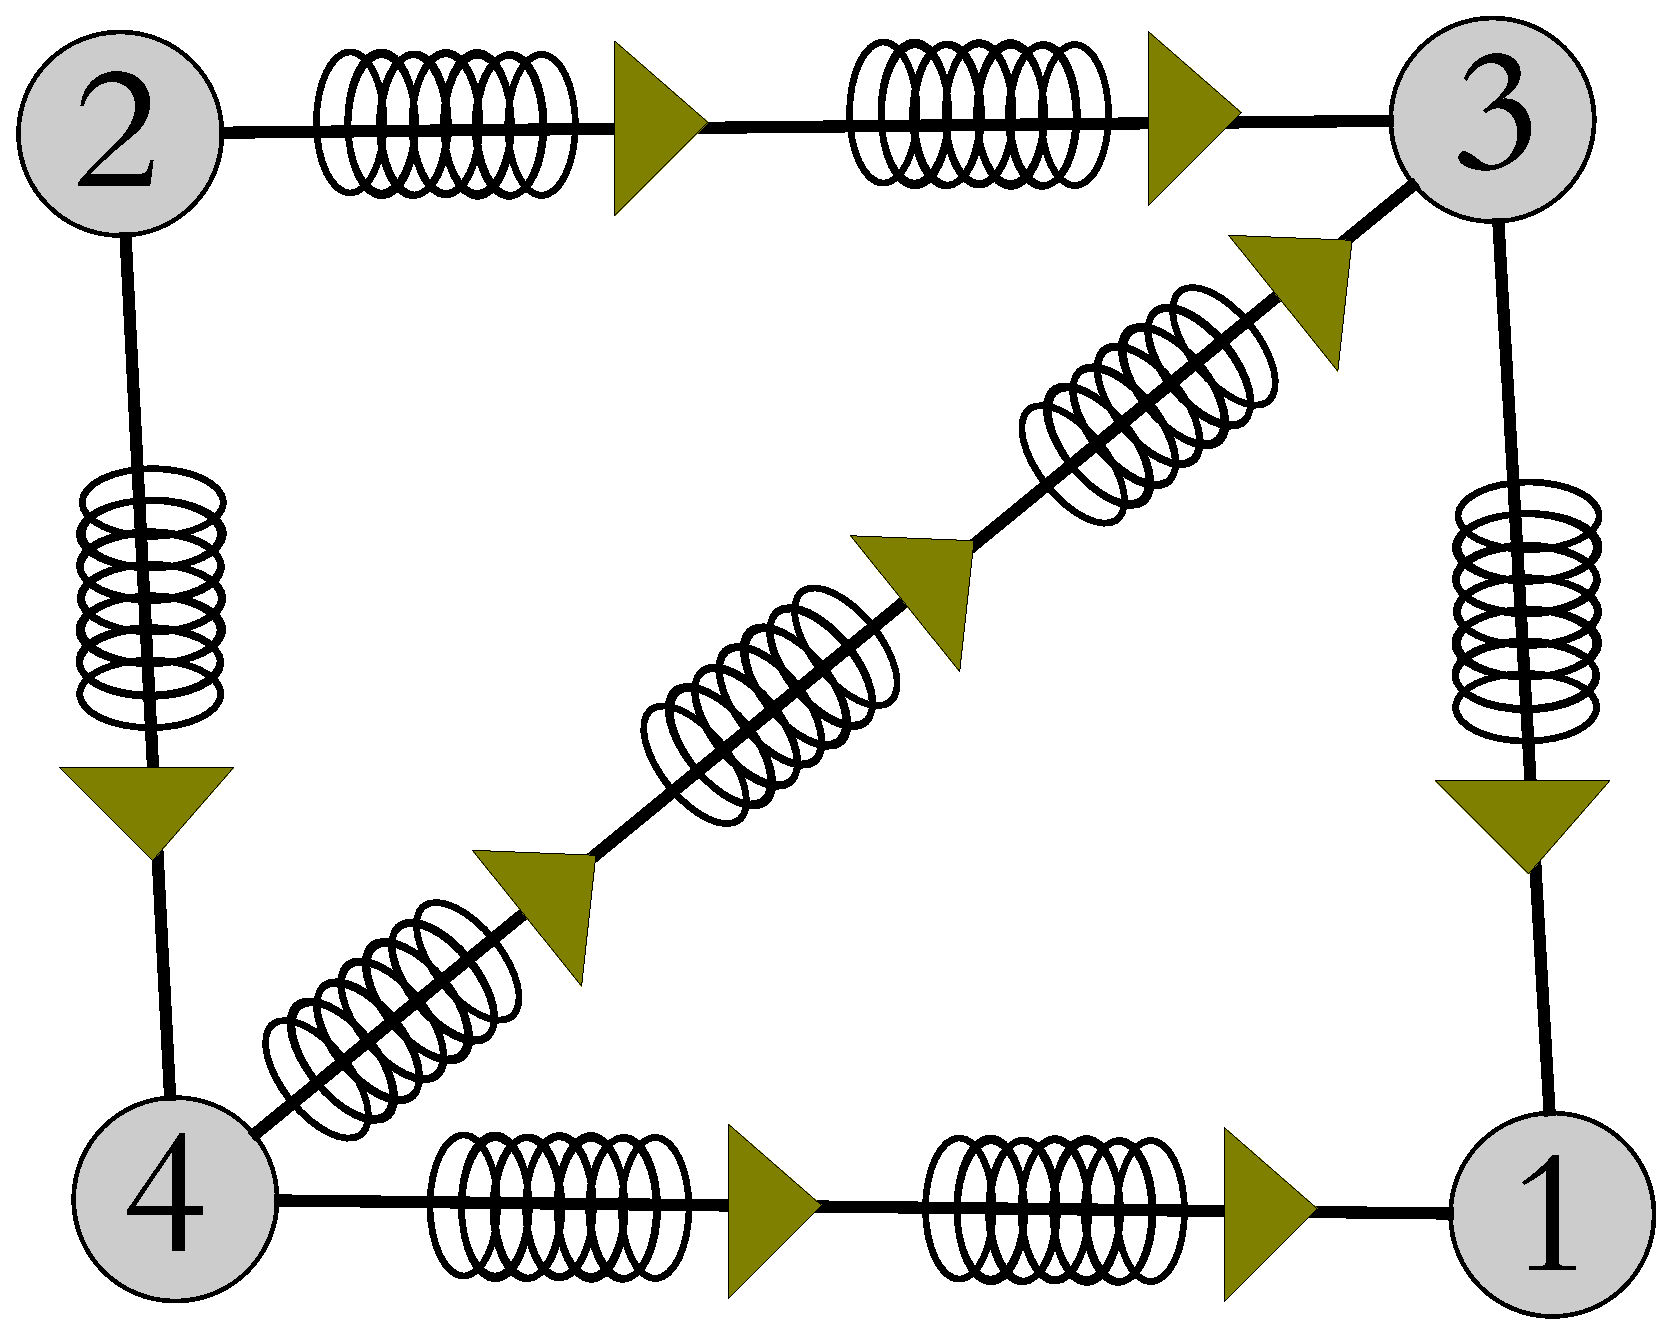
\includegraphics[scale=0.3]{PS1_Net}
%\end{figure}
\begin{enumerate}[label=\alph*)]
\item
A link is an entity connecting nodes. There are 5 links in the network.
\item
A span is an entity connecting amplifiers or nodes to amplifiers. There are 9 spans in the network.
\item
Node 1: deg = 2 , Node 2: deg = 2 , Node 3: deg = 3 , Node 4: deg = 3
\item
Nodes 1 and 3 have two pre-amplifiers each. Nodes 2 and 4 have two boosters each.
\end{enumerate}

%a. Which of the four tiers in an optical network (backbone [which is also called core or long-haul], regional, metro-core and access) are more cost-sensitive and what do you think about the reason?
%
%b. Mention some different technology implementations in tiers of an optical network and enrich your answer with enough explanations.
%
%c. What are the pros and cons of \textit{protocol and format transparency}?

\Q3

\begin{enumerate}[label=\alph*)]
\item
The problem of network engineering refers to the allocation of network resources to demands, prior to any routed demands. Typically, there is sufficient time between such plannings and running up the network based on them, whereas in traffic engineering, traffics are ongoing and any change in physical topology or arrival of a new traffic must be provised properly at a small time interval to prevent large latency.
\item
The client-side signal is created over 1310nm on spectrum, while network-side signals can vary over a range of wavelengths at the proximity of 1550nm (C-band). This generally requires a conversion between two different wavelengths which must exploit electronic devices rather than optical ones.
\item
Multiplexing refers to service multiplexing between two nodes and is performed at endpoints. Grooming enables multiplexing of multiple demands incident at any intermediate node (which requires more facilities for implementation) and allows a more optimal design, though more complicated.
\item
WSSs allow for configurable direction of wavelengths from input ports to output ports versus AWGs which provide a fixed wavelength pattern and limit the design. However, WSSs are more expensive.
\end{enumerate}

\Q4

Due to the symmetry of the network, we only need to calculate the number of wavelengths dropped or entered at nodes 1 to 6 according to the following topology:
\begin{figure}[h]
\centering
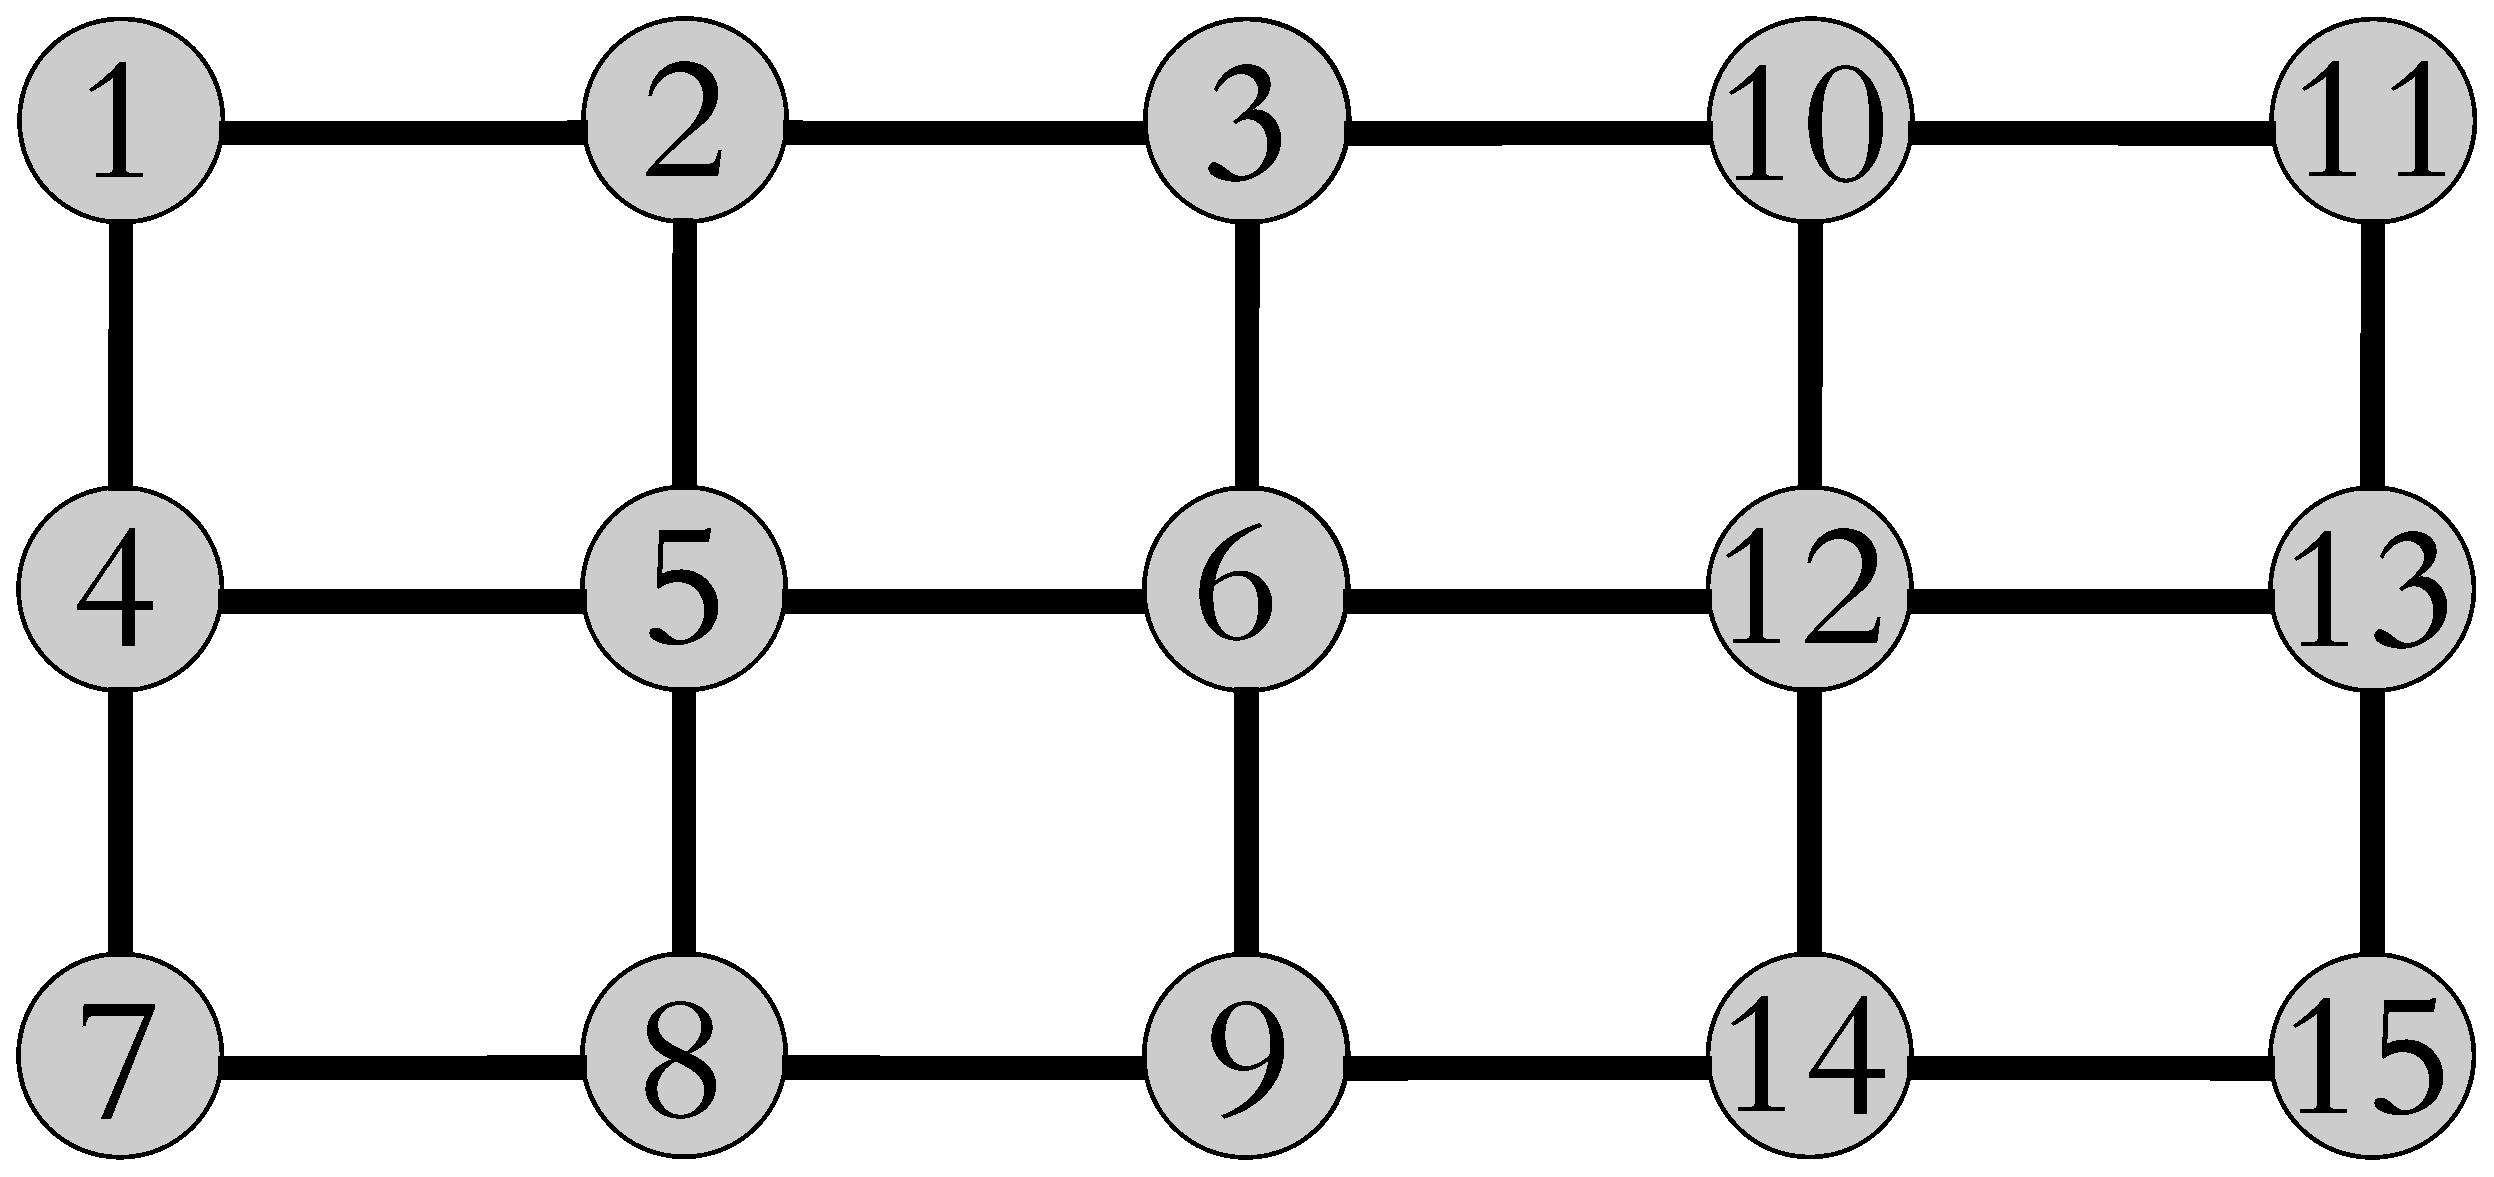
\includegraphics[width=80mm]{PS1_Net_num}
\end{figure}
Since optical reach is 3000km, all-optical connection can traverse at most 3 links between source and destination. We, therefore, assume here that all connections are at most 3-hops long.

For nodes 1, 2, 3, 4, 5 and 6, there are 8, 12, 13, 10, 13 and 15 number of wavelengths dropping, respectively. Hence the total number of dropped wavelengths anywhere in the network is equal to
\begin{equation}\begin{split}
&4\times \#(node1)
+
4\times \#(node2)
+
2\times \#(node3)
+
\\&
2\times \#(node4)
+
2\times \#(node5)
+
1\times \#(node6)
=
\\&
4\times 8+
4\times 12+
2\times 13+
%\\&
2\times 10+
2\times 13+
1\times 15
\\&=167
\end{split}\end{equation}
The number of wavelengths traversing nodes 1 to 6 without dropping is twice as much as the number of wavelengths traversing those nodes at each direction. Without loss of generality, we assume that the two shortest paths between two nodes at the two opposite directions form a rectabgle rather than being routed on equal nodes and links (the convention does not affect the solution since we are summing up the number of wavelengths at all nodes). An example of such a rectangle is the 1-2-3-6-5-4-1 rectangle where a connection from node 1 to node 6 is routed across nodes 2 and 3 and the opposite-direction connection from node 6 to node 1 is routed across nodes 5 and 4. These rectangles should be constituted of 6 links at most due to optical reach consideration. There are 10 rectangles with 6 links, 8 rectangles with 4 links, 6 rectangles with 3 links (such as 2-3-10-11) and 14 rectangles with two links (such as 1-2-3). The number of wavelengths traversed on these rectangles is equal to 8, 4, 4 and 2 respectively, yielding a total number of traversing wavelengths as
\begin{equation}\begin{split}
&8\times \#(\text{6-link rectangle})
+
4\times \#(\text{4-link rectangle})
+
\\&
4\times \#(\text{3-link rectangle})
+
%\\&
2\times \#(\text{2-link rectangle})
=
\\&
8\times 10+
4\times 8+
4\times 6+
%\\&
2\times 14
\\&=164,
\end{split}\end{equation}
giving the desired nodal drop ratio as $\frac{167}{167+164}\approx\%50.45$.

\Q5

\begin{enumerate}[label=\alph*)]
\item
No. The WDM output of the $M\times 1$ WSS (which is connected to the WDM input of $1\times N$ WSS) can carry one connection per wavelength. This restricts the cascade structure to not allowing two connections with different input and output ports to be carried on the same wavelength.
\item
Yes. A configuration for $M=2$ and $N=3$ is like
\begin{figure}[h]
\centering
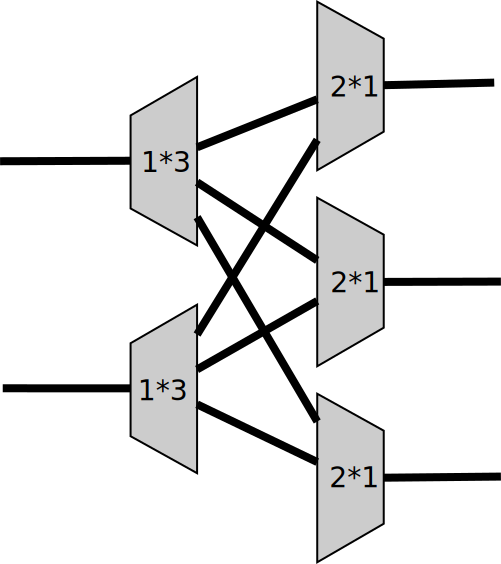
\includegraphics[width=60mm]{M_in_N_WSS}
\end{figure}
\item
In general, we need $M$ number of $1\times N$ and $N$ number of $M\times 1$ WSSs.
\end{enumerate}

\Q6

The structure with one splitter and multiple WSSs is more expensive with better wavelength isolation and multicast support (since WSS do not advertise a wavelength to multiple ports by default). In contrast, the structure with one WSS and many splitters advertises multiple wavelengths to a transponder which may cause a degrading in its filtering operation.

\Q7

\begin{enumerate}[label=\alph*)]
\item
The core switch must provide interconnection of $W$ wavelengths per degree and $WP$ wavelengths over the add/drop modules. Hence its size must be of order $NW+WP$.
\item
There are $WP$ add/drop modules required and the size of the edge switch would be of order $WP$.
\item
The ratio is equal to
$$
\frac{\text{size of edge switch}}{\text{size of core switch}}=\frac{WP}{WP+NW}=\frac{1}{1+N/P}.
$$
From the scalibility point of view, it is more efficient to have $N/P$ as minimal as possible (minimal degrees with maximal add/drop ratio).
\end{enumerate}

\end{document}